% Chapter 1

\chapter{Analisi} % Write in your own chapter title
\label{Chapter2}
\lhead{\emph{Analisi}}

\section{Il modello MOS}
\label{sec:mos}

In Fig. \ref{fig:simboliMos} il simbolo per un NMOS.

\begin{figure}[hbt!]
	\centering
	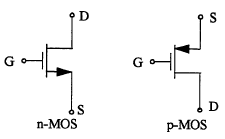
\includegraphics[width=0.5\textwidth]{figure/simboliMos.png}
	\caption{Simbolo NMOS (a sinistra) e PMOS (a destra)}
	\label{fig:simboliMos}
\end{figure}

L'Eq. \ref{eq:zonaSaturazione} descrive il comportamento di un MOS in zona di saturazione.

\begin{equation}
	I_{D} = \frac{1}{2} \mu _{n} C^{'}_{ox} \frac{W}{L} (V_{gs}-V_{th})^2
	\label{eq:zonaSaturazione}
\end{equation}

L'Eq. \ref{eq:formulaRapportoAspetto} è la relazione che consente di ricavare il rapporto d'aspetto necessario affinché il condensatore sia caricato/scaricato nel tempo desiderato.

\begin{equation}
\frac{W}{L} =
\begin{cases}
\frac{2C_{L}V_{DD}}{\tau \mu _{n} C^{'}_{ox} (V_{DD}-V_{thn})^2} \quad NMOS\\
\frac{2C_{L}V_{DD}}{\tau \mu _{p} C^{'}_{ox} (V_{DD}-|V_{thp}|)^2} \quad PMOS
\end{cases}
\label{eq:formulaRapportoAspetto}
\end{equation}

\section{Il Full Adder TSPC}
\label{sec:fullAdder}





